\section{Information problem}

	\subsection{Black hole radiation N} 
	%hawkings paper [1]
	\begin{figure}
		\begin{center}
			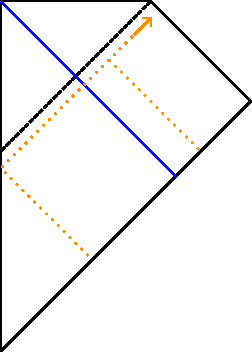
\includegraphics[scale=1]{collapse2}
			\caption{Bla} \label{plots_of_V}
		\end{center}
	\end{figure}

	\subsection{Entropy and thermodynamics \checkmark}
	If a black hole has a temperature and an energy, it must also have an entropy. So let's remember the inner energy in statistical mechanics\footnote{$\diff E = 
	T \diff S - p \diff V + \mu \diff N$} and derive it to:
		\begin{equation}
			\frac{\diff S}{\diff E} = \left. \frac{1}{T} \right|_{V,N=const.}
		\end{equation}
	For the black hole we have $T = \frac{1}{8 \pi G M}$ and $M=E$. If we assume that $S(E=0) = 0$, we can write:
		\begin{align}
			\frac{\diff S}{\diff M} &= 8 \pi G M \nonumber \\
			&\Leftrightarrow \int_0^S \diff S' = \int_0^M 8 \pi M' dM' \nonumber\\
			&\Leftrightarrow S = 4 \pi G M^2 & & \Bigm| r_s = 2GM \nonumber\\
			&\Leftrightarrow S = \frac{r_s^2 \pi}{G}  & & \Bigm| A=4 \pi r_s^2 \text{~and~} l_p = \sqrt{8 \pi G} \nonumber\\
			\Leftrightarrow~
			S &= \frac{A}{4G} = 2 \pi \frac{A}{l_p} \label{entropy}
		\end{align}
	For a black hole of the mass of our sun, this entropy would be $10^{78}$ which is enormous! If we take the sun like it is, the entropy would ``just'' be $10^{60}$. 
	
	Historical the entropy of a black hole was discovered before its temperature. With help of classical general relativity, we can see that the area of an event horizon of a black hole never decreases which looks quite like the second law of thermodynamics. Together with certain formal definition of the entropy, where it is proportional to the horizon area and a temperature indirect proportional to the Schwarzschild radius, the first law of thermodynamics with $\diff M = T \diff S$ is satisfied, too. 
	
	Jacob Bekenstein was holding out that this entropy should be that kind of statistical entropy of a black hole, that counts the number of ways it could have formed itself. 
	In a thought experiement he was throwing some systems with own entropy into a black hole and discovered that the interior entropy was growing faster, than the exterior entropy was sinking because of the systems loss. 
	So this means, that the entropy must be given by some constant proportional to the horizon area in Planck units.
	Bekenstein called this the \textit{Genereralized Second Law}.
	
	As Hawking published his paper about the temperature of a black hole, Bekensteins theory strongly reinforced. This is why the entropy of a black hole is often called \textbf{Bekenstein-Hawking entropy}. 
	
	In \textit{string theory} this idea of an entropy counting microstates is strong supported. For example in many situations where we count the states of a long vibrating string we can see how big the entropy of a black hole is. In some supersymmetric cases it is even possible to compute the $\frac{1}{4}$ in equation \eqref{entropy}.
	
	\subsection{Evaporation N}
	%hawkings paper [2]

	%\clearpage
	\subsection{What happens to the information while evaporation? N}
	Steven Hawking said in his paper\marginpar{[2]}, it is inconsistent with quantum mechanics, that the black hole's entropy counts the number of ways it could have been formed which most people would think in the first place. 
	
	The idea behind these thoughts is that the outgoing radiation of a black hole is completely independent of details of the initial state of photons. 
	In explicit we make a diagonal density matrix
		\begin{equation} \label{density matrix informprobl}
			\rho \propto \bigotimes_{\omega, l, m} \left(
			\sum_n \ket{n} \bra{n}_{\omega, l, m} P_{abs} (\omega, l) e^{-\beta \omega n}
			\right)
		\end{equation}
	which leads to the emission rate\marginpar{das gehört weiter nach oben} 
		\begin{equation}
			\frac{\diff E}{\diff t} = 
			\frac{\omega \diff \omega}{2\pi} 
			\frac{P_{abs}(\omega, l)}{e^{\beta \omega}-1}
		\end{equation}
	where $\beta = \frac{1}{T_{Hawking}}$, and $P_{abs}(\omega, l)$ is the absorption
	probability of a ``blue'' mode.
		
	This should remind you of the Rindler result which means that this reduced density matrix for the right or left Rindler wedge is just a thermal density matrix. But back then, we did not calculate in the gravity, so there will be catastrophic consequences once we turn on the gravity again.
		
	Now, if a black hole was orginally formed in some pure state $\ket{\psi}$, its outside radiation field becomes more and more mixed as we move forward in time. Because we are normally only looking at the late radiation outside of the black hole, this doesn't seem problematic. 
		
	While the black hole evaporates and becomes smaller, its entanglement entropy is always increasing as seen in \eqref{density matrix informprobl}. The problem is, its size decreases until it is Planckian\footnote{The planck scale begins at the planck length $l_p = \sqrt{\frac{\hbar G}{c^3}} \approx 1,6 \cdot 10^{-35}\unit{m}$, while a proton is about the size of $8,4 \cdot 10^{-16}\unit{m}$} and in those kinds of systems our common physics can't help us any more.
	
	What happens to the entropy now? One of two things must happen:
		\begin{enumerate}[(1)]
			\item The evaporation stops at Planck size. This rest is also called ``remnant'' and its entanglement entropy must be enormously big, bigger than that of a black hole with a comparable mass. \label{evap. planck size}
			\item The black hole finishes the evaporation till there is nothing left. The law of energy conservation prohibits that the last boost of photons contains enough entanglement entropy for reproducing the initial state. But if information can not get lost, we would have to violate the quantum mechanics here.
			So in the end we would have a mixed state with an entropy comparable to the one of the initial horizons entropy. \label{evap. finished}
		\end{enumerate}
	The option number \eqref{evap. planck size} is in fact possible, but it would mean that there are objects with an infinit amount of states below any finite energy.
	Also if a black hole can form out of photons and gravitons why should it not be possible for it to disapear entirely back into photons and gravitons.
	
	Option \eqref{evap. finished} in contrast seems to be the better choice, but it also means that black holes can destroy information. So one must admitt that gravity and quantum mechanics are inconstistent, they have no theory in common.
	
	Let's have a look at an other option, which is nearly similar to option number \eqref{evap. finished}:
		\begin{enumerate}[(3)]
			\item While evaporating, the information is hidden in some entanglement between the Hawking photons blasted by the black hole (or the rest of it).
			In the end we have a pure state of the radiation field instead of a mixed state like in \eqref{evap. finished}. This is just possible if we don't look at too many photons at once, because in complicated states any small subsystem looks thermal, so it can justify \eqref{density matrix informprobl}. 		
		\end{enumerate}				
		